\documentclass[11pt]{beamer}
\usetheme{Warsaw}
\usepackage[utf8]{inputenc}
\usepackage[vietnamese]{babel}
\usepackage{amsmath}
\usepackage{amsfonts}
\usepackage{amssymb}
\usepackage{graphicx}
\usepackage{caption}
\usepackage{booktabs}

%
\author{Vương Gia Bảo, Nguyễn Viết Dũng, Ngô Xuân Kiên, Lê Nhựt Nam}
\title{NHẬP MÔN MÁY HỌC \newline  TRÌNH BÀY VỀ BÀI BÁO "Speaker Recognition from Raw Waveform with SincNet"}
\institute{Đại học Khoa học Tự nhiên, Đại học Quốc gia TP HCM} 


%
\setbeamertemplate{caption}[numbered]
% \setbeamertemplate{footline}[frame number]
% footer
\makeatletter
\setbeamertemplate{footline}
{
	\leavevmode%
	\hbox{%
		\begin{beamercolorbox}[wd=1\paperwidth,ht=2.25ex,dp=1ex,right]{institute in head/foot}%
			\usebeamerfont{title in head/foot} 
			\insertframenumber{} / \inserttotalframenumber\hspace*{2ex} 
	\end{beamercolorbox}}%
}
\makeatother
%
\newcommand{\argmax}{\arg\!\max}

\begin{document}

\begin{frame}
\titlepage
\end{frame}

\begin{frame}{Nội dung trình bày}
\tableofcontents
\end{frame}


\section{Động lực nghiên cứu khoa học}
\begin{frame}{Động lực nghiên cứu khoa học}
	\begin{itemize}
		\item Về lĩnh vực Nhận dạng giọng nói, đây là một lĩnh vực nghiên cứu có nhiều ứng dụng vào thực tiễn đời sống như xác thực sinh trắc học, pháp y, bảo mật, nhận dạng giọng nói và phân cực giọng nói.
		\item Các phương pháp SOTA dựa trên việc biểu diễn i-vectors của những đoạn
		giọng nói, cải thiện đáng kể so với mô hình Gaussian Mixture Model-Universal Background Models
		\item Sự phát triển của Deep Neural Networks
	\end{itemize}
\end{frame}

\section{Phát biểu bài toán}
\begin{frame}{Phát biểu bài toán}
	Hai tác vụ lớn trong lĩnh vực Nhận dạng Giọng nói:\newline
	\begin{itemize}
		\item Tác vụ: Định danh người nói (Speaker Identification)
		\begin{itemize}
			\item Đầu vào (Input): Dữ liệu âm thanh giọng nói
			\item Đầu ra (Output): Danh tính của người nói
		\end{itemize}
		\item 	Tác vụ: Xác minh người nói (Speaker Verification)
		\begin{itemize}
			\item Đầu vào (Input): Dữ liệu âm thanh giọng nói
			\item Đầu ra (Output): Đồng ý/ Từ chối
		\end{itemize}
	\end{itemize}
\end{frame}
\section{Giới thiệu về bài báo}
\begin{frame}{Giới thiệu về bài báo}
	\begin{itemize}
		\item Bài báo đề xuất một kiến trúc mạng CNN (Convolutional Neural Networks) mới, khai phá lớp tích chập đầu tiên để khám phá nhiều thông tin hơn - SincNet.
		\item SincNet dựa trên các hàm sinc được tham số hóa, để cài đặt các bộ lọc băng thông.
		\item Ngược lại với CNNs chuẩn, học tất cả các phần tử của mỗi bộ lọc filter, ở đây, SincNet chỉ dùng các tần số cắt thấp và cao học trực tiếp dữ liệu với phương pháp đề xuất.
		\item Nhỏ gọn và hiệu quả trong việc tùy chỉnh với ứng dụng mà chúng ta muốn.
		\item Sự kết hợp tuyệt vời giữa Học máy (Machine Learning) và Xử lý Tín hiệu số (Digital
		Signal Processing).
	\end{itemize}
\end{frame}

\section{Vấn đề khi xử lý tín hiệu giọng nói}
\begin{frame}{Vấn đề khi xử lý tín hiệu giọng nói}
	\begin{itemize}
		\item Dữ liệu với số chiều cao
		\begin{figure}[H]
			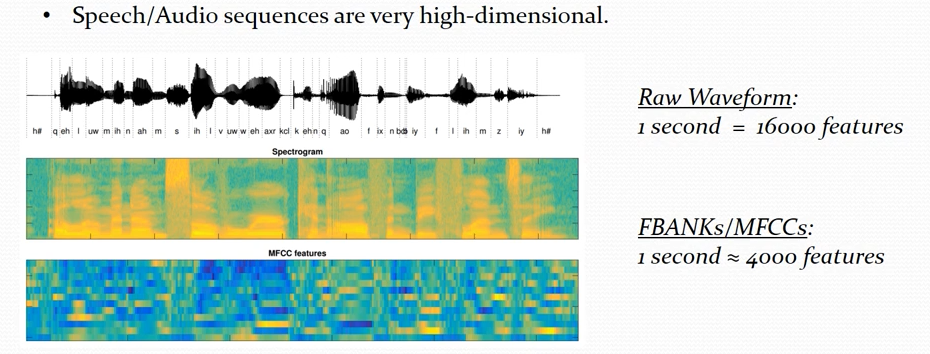
\includegraphics[width=1\linewidth]{images/capture_01.png}
			\caption{A brief introduction to SincNet - Mirco Ravanelli}
			\label{fig:writing-thesis}
		\end{figure}
	\end{itemize}
\end{frame}
\begin{frame}{Vấn đề khi xử lý tín hiệu giọng nói}
	\begin{itemize}
		\item Sự biến mất độ dốc đạo hàm - vanishing gradient
		\begin{figure}[H]
			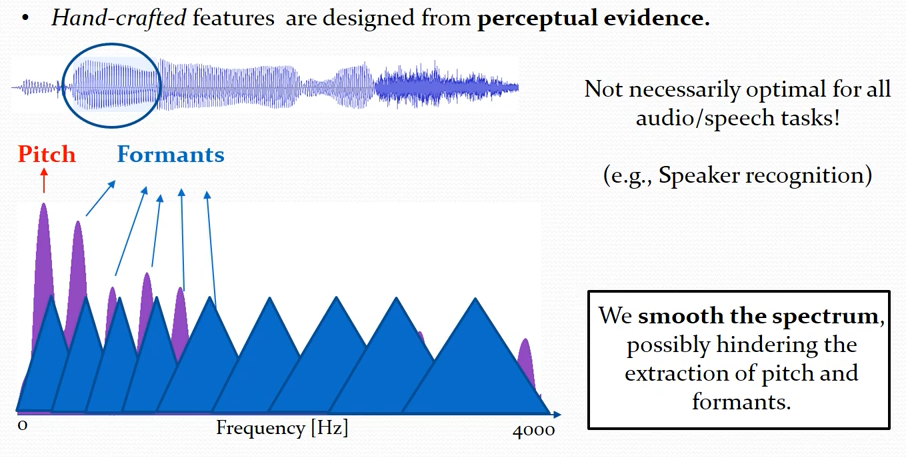
\includegraphics[width=0.9\linewidth]{images/perceptual_evidence.png}
			\caption{A brief introduction to SincNet - Mirco Ravanelli}
			\label{fig:writing-thesis}
		\end{figure}
	\end{itemize}
\end{frame}
\begin{frame}{Vấn đề khi xử lý tín hiệu giọng nói}
	\begin{itemize}
		\item Các bộ lọc CNNs thường có những hình dạng đa băng tần không hợp lý, khó hiểu với con người.
		\begin{figure}[H]
			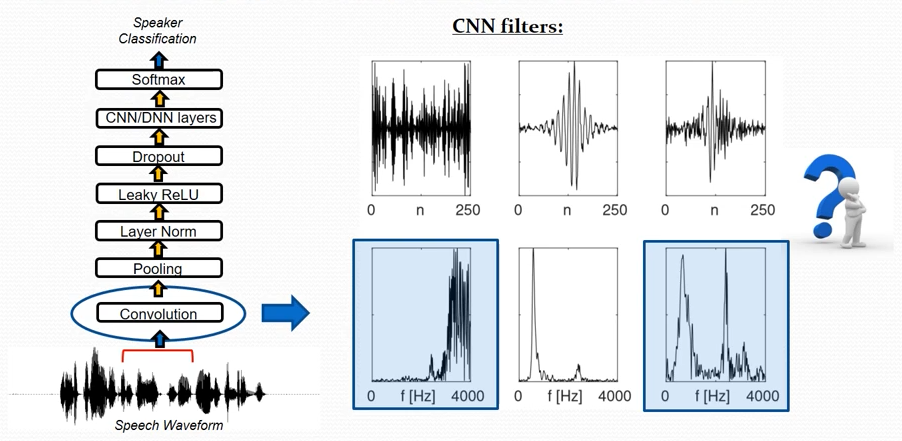
\includegraphics[width=0.9\linewidth]{images/interpretability_problems.png}
			\caption{A brief introduction to SincNet - Mirco Ravanelli}
			\label{fig:writing-thesis}
		\end{figure}
	\end{itemize}
\end{frame}

\section{Kiến trúc mạng SincNet}
\begin{frame}{SincNet}
	\begin{block}{~\vspace{0.7cm}}
		\begin{center}
			\vspace{-0.8cm}
			\begin{tabular}{p{0.45\textwidth}|p{0.45\textwidth}}
				\textcolor{white}{\bf Standard CNN} & \textcolor{white}{\bf SincNet} \\\\
				 $y[n] = x[n] * h[n]$ & $y[n] = x[n] * g[n, \theta]$\\
				 Học từ tất cả các phần tử của mỗi filter & Chỉ học từ tham số $\theta$ của một kernel được định nghĩa từ trước\\
			\end{tabular}
		\end{center}
	\end{block}
	\textbf{Vấn đề đặt ra: Làm thế nào để chọn được hàm $g(.)$?}
\end{frame}
\begin{frame}{SincNet}
	Ý tưởng để xây dựng hàm $g(.)$ đến từ Xử lý tín hiệu số, dựa trên bộ lọc băng thông (\textbf{band-pass filters}), chỉ có tần số cắt thấp và cao (low-high cutoff frequencies) được học
	\begin{figure}[H]
		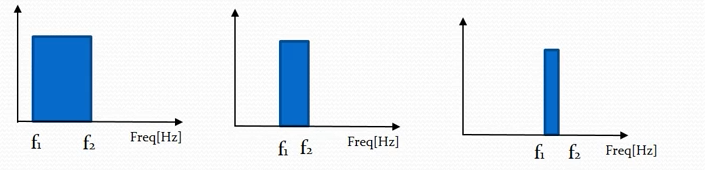
\includegraphics[width=0.9\linewidth]{images/band_passfilters.png}
		\caption{A brief introduction to SincNet - Mirco Ravanelli}
		\label{fig:writing-thesis}
	\end{figure}
\end{frame}
\begin{frame}{SincNet}
	Với $f_1$ $f_2$ lần lượt là tần số cắt thấp (low) và cao (high) đã được học, $rect(.)$ là hàm rectangular trong miền tần số.
	
	$$G[f, f_1, f_2] = rect\left(\frac{f}{2f_2}\right) -  rect\left(\frac{f}{2f_1}\right)$$
	
	Để có thể trở lại miền thời gian được, ta sử dụng phép biến đổi Fourier Ngược. Thu được
	
	$$g[n, f_1, f_2] = 2f_2sinc(2\pi f_2 n) - 2f_1sinc(2\pi f_1 n)$$ 
\end{frame}
\begin{frame}{SincNet}
	\begin{block}{~\vspace{0.7cm}}
		\begin{center}
			\vspace{-0.8cm}
			\begin{tabular}{p{0.45\textwidth}|p{0.45\textwidth}}
				\textcolor{white}{\bf CNN Filters} & \textcolor{white}{\bf SincNet Filters} \\\\
				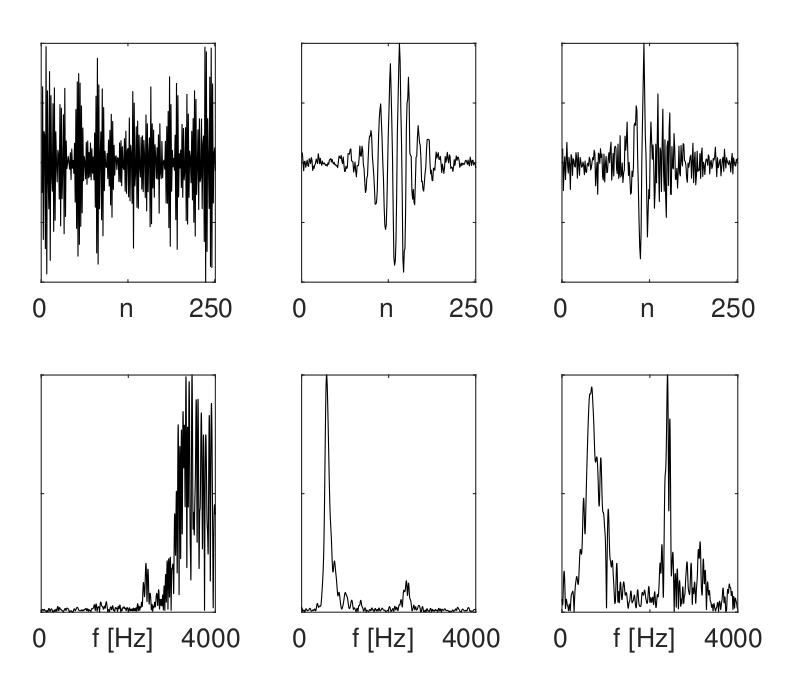
\includegraphics[width=1\linewidth]{images/cnn_filters.png} & 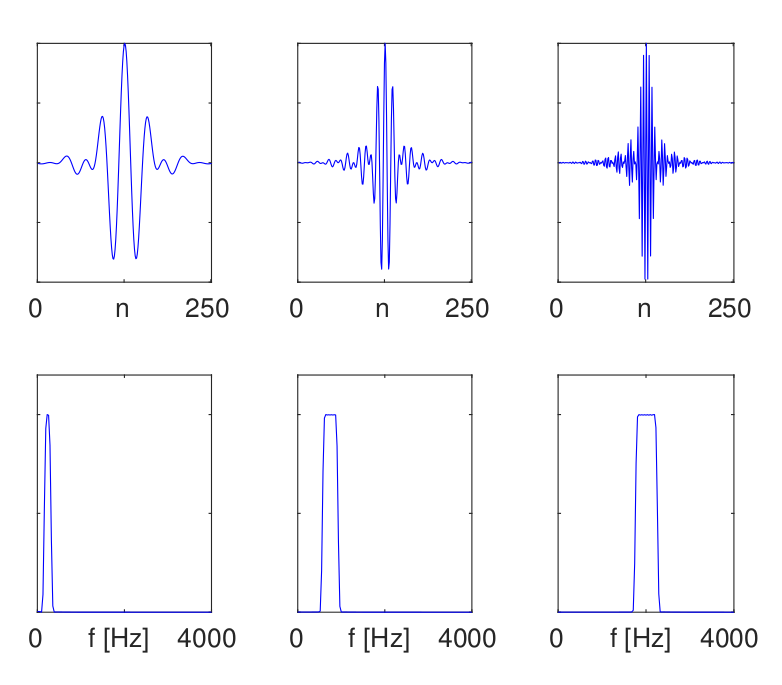
\includegraphics[width=1\linewidth]{images/sincnet_filters.png}\\
			\end{tabular}
		\end{center}
	\end{block}
\end{frame}
\begin{frame}{Kiến trúc mạng SincNet}
	\begin{figure}[H]
		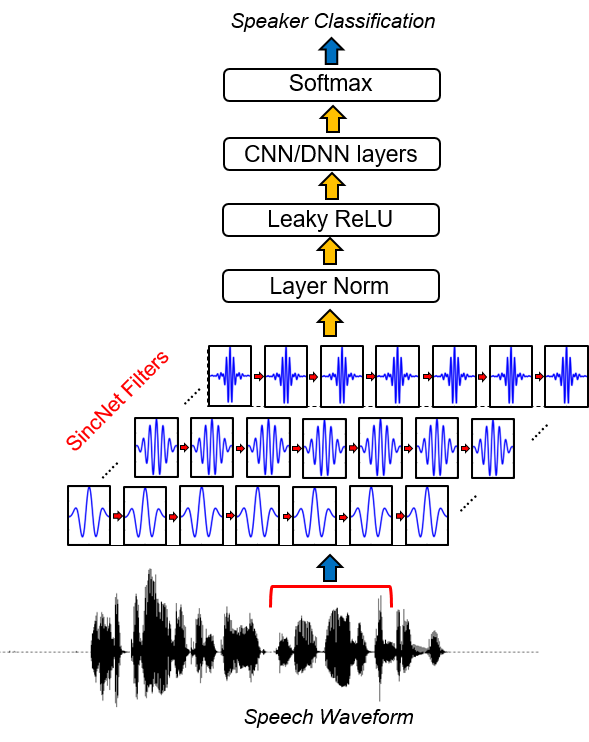
\includegraphics[width=0.4\linewidth]{images/SincNet.png}
		\caption{The SincNet Architecture}
		\label{fig:writing-thesis}
	\end{figure}
\end{frame}
\begin{frame}{Đặc điểm mô hình mạng SincNet}
	\begin{columns}
		\begin{column}{0.47\textwidth}
			\begin{figure}[H]
				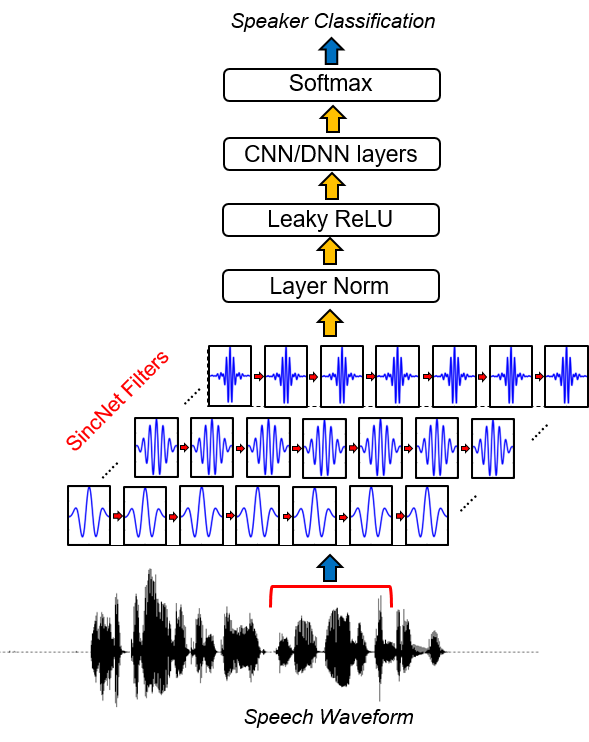
\includegraphics[width=0.9\linewidth]{images/SincNet.png}
			\end{figure}
		\end{column}
		\begin{column}{0.5\textwidth}
		\begin{itemize}
			\item Tính hội tụ nhanh
			\begin{figure}[H]
				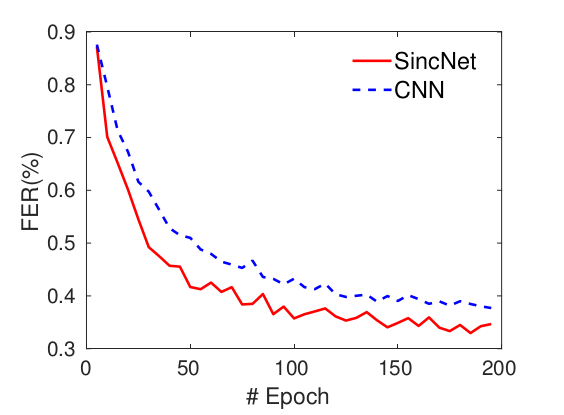
\includegraphics[width=0.9\linewidth]{images/fast_convergence.png}
			\end{figure}
		\end{itemize}
		\end{column}
	\end{columns}
\end{frame}
\begin{frame}{Đặc điểm mô hình mạng SincNet}
	\begin{columns}
		\begin{column}{0.47\textwidth}
			\begin{figure}[H]
				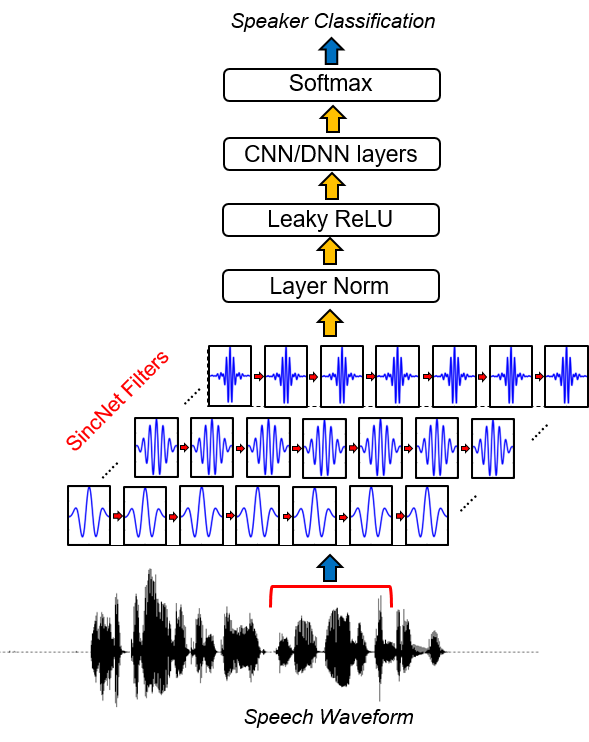
\includegraphics[width=0.9\linewidth]{images/SincNet.png}
			\end{figure}
		\end{column}
		\begin{column}{0.5\textwidth}
			\begin{itemize}
				\item Tính hiệu quả
				\begin{figure}[H]
					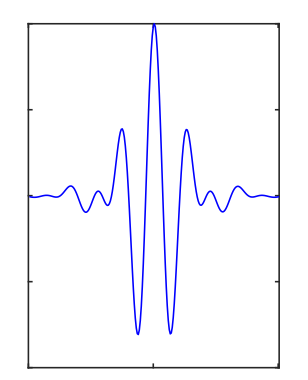
\includegraphics[width=0.45\linewidth]{images/g_symmetric.png}
				\end{figure}
				\item 	Các hàm kernel $g(.)$ là đối xứng nên chỉ cần thực hiện phép tích chập trên một phần filter. 
				\item Điều này sẽ tiết kiệm 50\% việc tính toán.
			\end{itemize}
		\end{column}
	\end{columns}
\end{frame}
\begin{frame}{Đặc điểm mô hình mạng SincNet}
	\begin{columns}
		\begin{column}{0.47\textwidth}
			\begin{figure}[H]
				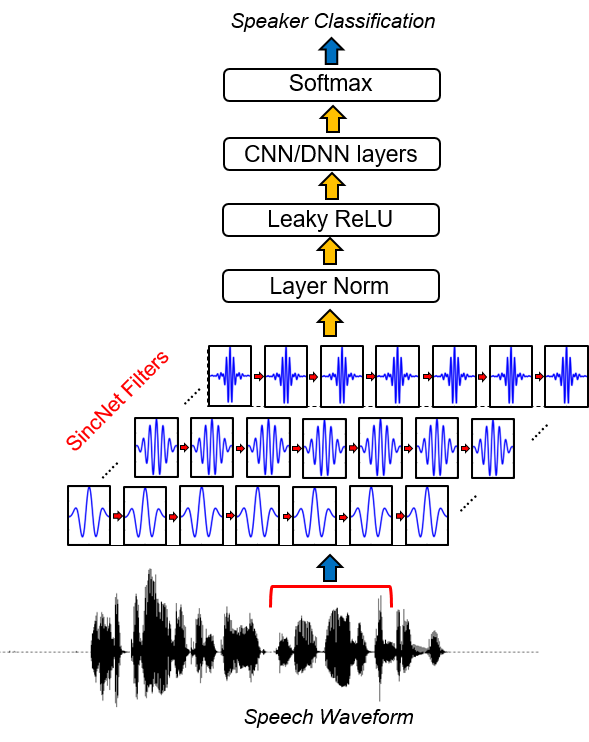
\includegraphics[width=0.9\linewidth]{images/SincNet.png}
			\end{figure}
		\end{column}
		\begin{column}{0.5\textwidth}
			Cần ít tham số cho việc huấn luyện mô hình. \newline
			Giả sử ta gọi: $F$ là số bộ lọc filters, $L$ kích thước của mỗi bộ lọc  filters
			\begin{itemize}
				\item Với CNN, số tham số là $parameters = F * L$
				\item Với SincNet, số tham số là $parameters = 2F$
			\end{itemize}
		\end{column}
	\end{columns}
\end{frame}
\begin{frame}{Đặc điểm mô hình mạng SincNet}
	\begin{columns}
		\begin{column}{0.47\textwidth}
			\begin{figure}[H]
				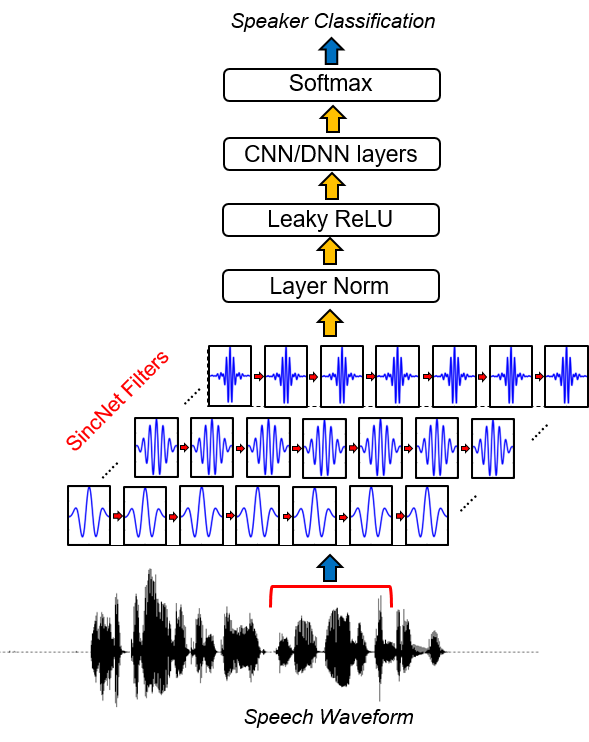
\includegraphics[width=0.9\linewidth]{images/SincNet.png}
			\end{figure}
		\end{column}
		\begin{column}{0.5\textwidth}
			\begin{itemize}
				\item Tính giải nghĩa/ diễn giải
				\begin{figure}[H]
					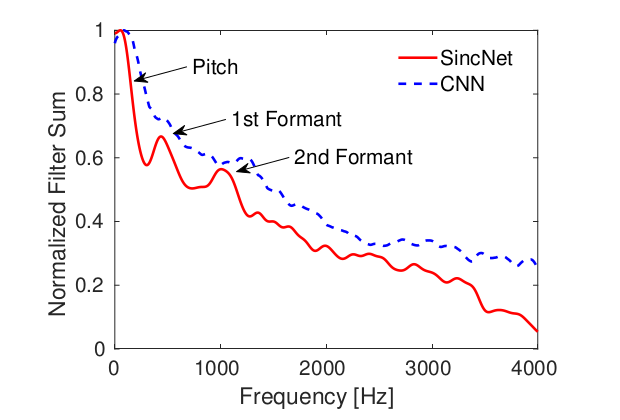
\includegraphics[width=0.9\linewidth]{images/interpretability.png}
				\end{figure}
			\end{itemize}
		\end{column}
	\end{columns}
\end{frame}

\section{Các kết quả}
\begin{frame}{Các kết quả đối với tác vụ Speaker Identification}
\begin{figure}[H]
	\centering
	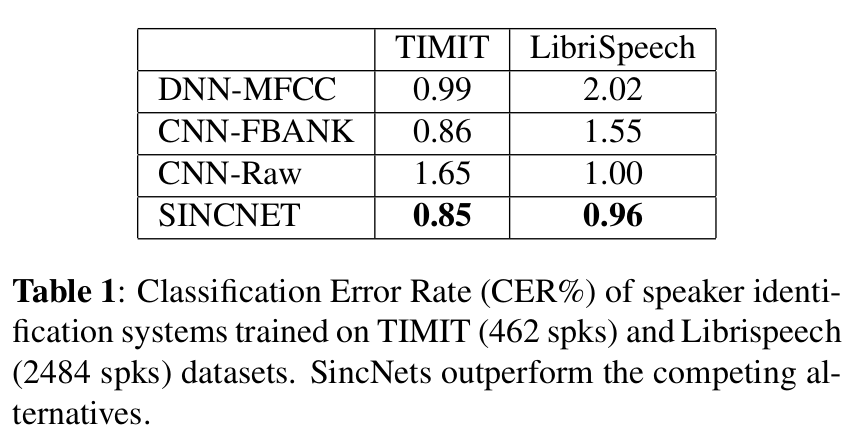
\includegraphics[width=0.75\textwidth]{images/performance_speaker_identification.png}
	\caption{Bảng kết quả SicNet trong tác vụ nhận dạng giọng nói - SI}
	\label{fig:writing-thesis}
\end{figure}	
\end{frame}
\begin{frame}{Các kết quả đối với tác vụ Speaker Verification}
\begin{figure}[H]
	\centering
	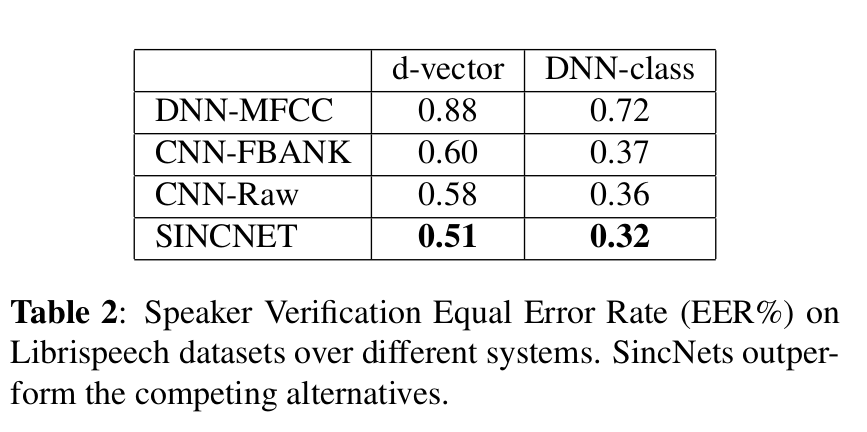
\includegraphics[width=0.75\textwidth]{images/performance_speaker_verification.png}
	\caption{Bảng kết quả SicNet trong tác vụ xác minh giọng nói - SV}
	\label{fig:writing-thesis}
\end{figure}	
\end{frame}
\begin{frame}{Các kết quả đối với tác vụ SV i-vectors}
	Hệ thống \textbf{i-vector} tốt nhất của nhóm tác giả đạt được \textbf{EER = 1,1\%}, \textbf{khá xa so với những gì đạt được với hệ thống DNN}.	
\end{frame}
\begin{frame}{Kết quả Speaker Recognition trên DIRHA}
	\begin{figure}[H]
		\centering
		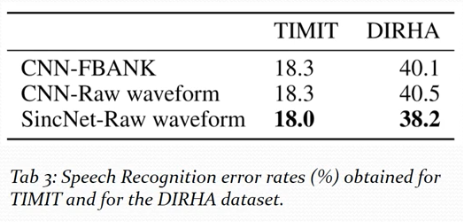
\includegraphics[width=0.65\textwidth]{images/sr_sincnet_result.png}
		\caption{Bảng kết quả Speaker Recognition SincNet trên tập DIRHA}
		\label{fig:writing-thesis}
	\end{figure}
	SincNet hoạt động rất tốt trên DIRHA, so với các kỹ thuật khác, nó luôn có độ lỗi thấp nhất.	
\end{frame}

\section{Kết luận}
\begin{frame}{Kết luận}
	Về SincNet Architecture
	\begin{itemize}
		\item Cơ sở lý thuyết Toán học vững vàng: Kỹ thuật band-pass filter, Window trong Xử lý tín hiệu số.
		\item Tính toán nhanh và gọn nhẹ: Như đã nói, đây là một đặc điểm của SincNet nhờ vào dùng ít tham số, kernel đối xứng.
		\item Kết hợp với Deep Learning một cách hiệu quả.
		\item Sử dùng DNN-Class trong đánh giá, cho kết quả đầy hứa hẹn, có độ lỗi EER thấp
	\end{itemize}
	Nhưng vẫn có hạn chế
	\begin{itemize}
		\item DNN-class tuy có EER thấp nhưng đánh đổi nhiều sự linh hoạt so với d-vectors
	\end{itemize}
\end{frame}

\section{Tài liệu tham khảo}
\begin{frame}{Tài liệu tham khảo}
	\nocite{*}
	\bibliography{references}\newpage\cleardoublepage
	\bibliographystyle{plain}
\end{frame}


\begin{frame}{Q\&A}
	\begin{center}
		\Huge Cảm ơn thầy và các bạn đã theo dõi và lắng nghe
	\end{center}
\end{frame}

\end{document}